\section{Background}

% \begin{frame}{Outline}
% \tableofcontents[currentsection]
% \end{frame}

\begin{frame}{Regularization Alleviate Overfitting}

% Regularization is the most important approach in practice to alleviate overfitting and improve generalization. The following figures sketch the generalization behaviour of the deep neural networks.

% Typical regularization techniques improve generalization through various approaches, including:

% However, more {\bf principled} and more {\bf powerful} regularization schemes are yet to be discovered.

Effective regularization schemes alleviate overfitting and improve generalization.

\begin{figure}
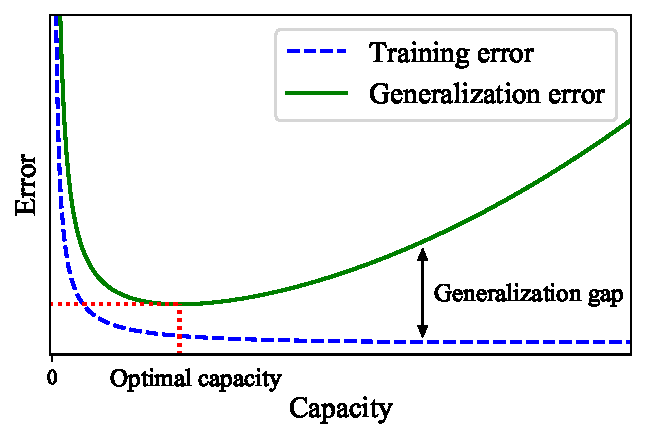
\includegraphics[width=.45\textwidth]{figs/gap1.pdf}
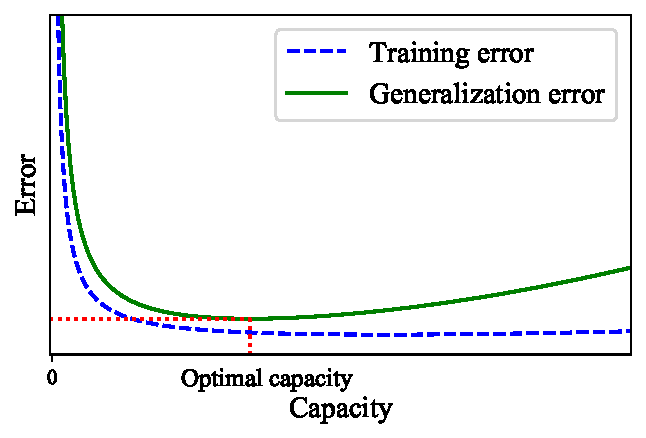
\includegraphics[width=.45\textwidth]{figs/gap2.pdf}
\end{figure}
\vspace{-1em}
{\small
\begin{itemize}
    \item Some researchers have found the modern neural networks may have a different behaviour, \ie, the {\em Double Descent} (Nakkiran \etal, 2020). Nevertheless, well-regularized neural networks consistently achieve better performance in practice.
\end{itemize}
}

\end{frame}

\begin{frame}{Flat Minima Helps Generalization}

\begin{itemize}
    \item Flat minima correspond to low-complexity networks. (Hochreiter \etal, 1997)
    \item Small-batch SGD produces flat minima that generalize well. (Keskar \etal, 2017)
    \item Better minimizers of loss function are flatter in visualization. (Li \etal, 2018)
    \item A PAC-Bayes based generalization guarantee for flat minima. (Foret \etal, 2020)
\end{itemize}

\begin{figure}
\subcaptionbox{ResNet without skip connections}[.48\textwidth]{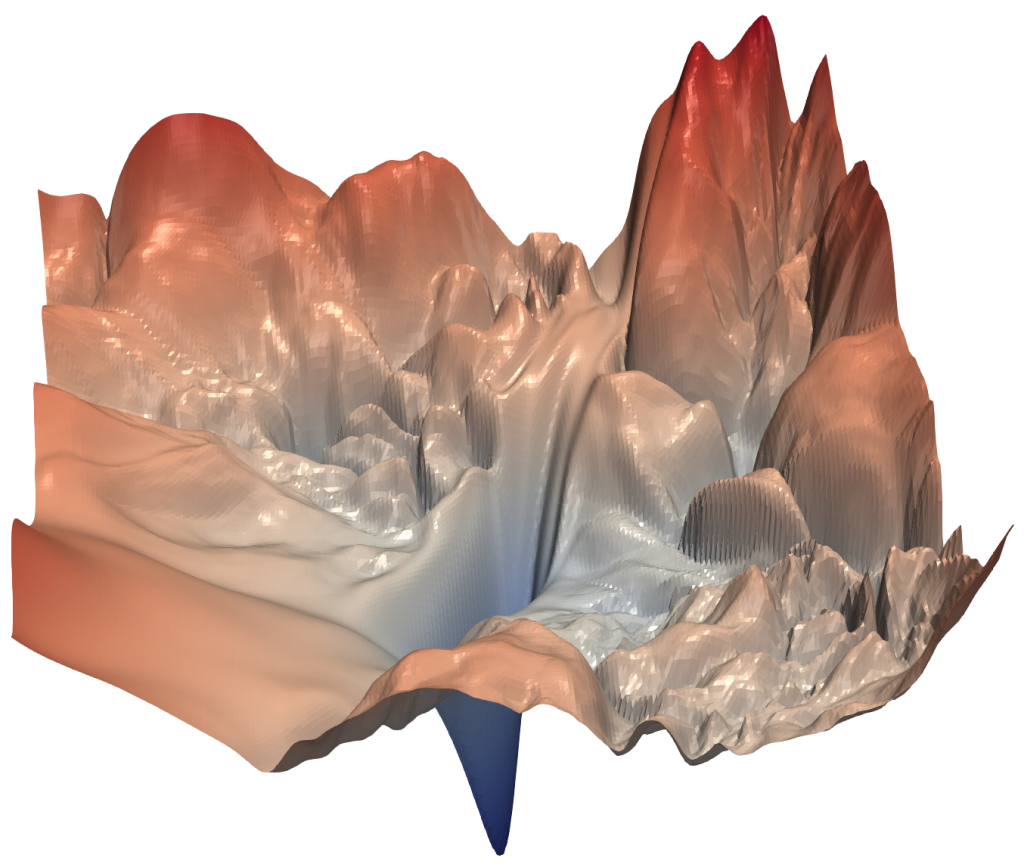
\includegraphics[width=.25\textwidth]{figs/flatness_a.png}}
\subcaptionbox{ResNet with skip connections (Li \etal, 2018)}[.48\textwidth]{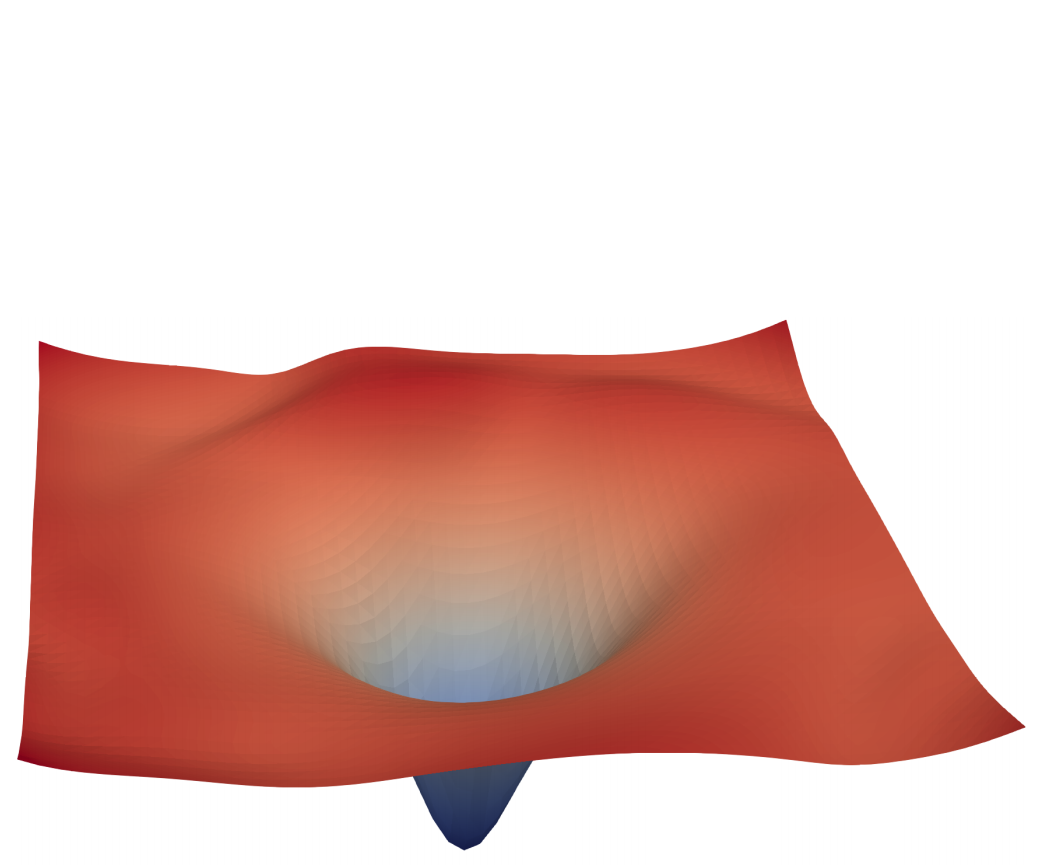
\includegraphics[width=.25\textwidth]{figs/flatness_b.png}}
\end{figure}
\end{frame}
